% !TEX TS-program = XeLaTeX
% use the following command:
% all document files must be coded in UTF-8
\documentclass[portuguese]{textolivre}
% build HTML with: make4ht -e build.lua -c textolivre.cfg -x -u article "fn-in,svg,pic-align"

\journalname{Texto Livre}
\thevolume{16}
%\thenumber{1} % old template
\theyear{2023}
\receiveddate{\DTMdisplaydate{2023}{7}{12}{-1}} % YYYY MM DD
\accepteddate{\DTMdisplaydate{2023}{9}{24}{-1}}
\publisheddate{\DTMdisplaydate{2023}{11}{10}{-1}}
\corrauthor{Antía Cores Torres}
\articledoi{10.1590/1983-3652.2023.46865}
%\articleid{NNNN} % if the article ID is not the last 5 numbers of its DOI, provide it using \articleid{} commmand 
% list of available sesscions in the journal: articles, dossier, reports, essays, reviews, interviews, editorial
\articlesessionname{Articles}
\runningauthor{Barbosa et al.} 
%\editorname{Leonardo Araújo} % old template
\sectioneditorname{Daniervelin Pereira}
\layouteditorname{Leonado Araújo}

\title{Materiais didáticos digitais para o ensino/aprendizagem das ciências naturais: uma análise bibliométrica}
\othertitle{Digital didactic materials for the teaching/learning of the natural sciences: a bibliometric analysis}
% if there is a third language title, add here:
%\othertitle{Artikelvorlage zur Einreichung beim Texto Livre Journal}

\author[1]{Mayara Lustosa de Oliveira Barbosa~\orcid{0000-0003-3356-0998}\thanks{Email: \href{mailto:mayara.barbosa@ifb.edu.br}{mayara.barbosa@ifb.edu.br}}}
\author[2]{Diana Marín-Suelves~\orcid{0000-0002-5346-8665}\thanks{Email: \href{mailto:diana.marin@uv.es}{diana.marin@uv.es}}}
\author[3]{Cecilia V. Becerra-Brito~\orcid{0000-0002-2283-4001}\thanks{Email: \href{mailto:cbecerra@ull.edu.es}{cbecerra@ull.edu.es}}}
\author[4]{Antía Cores Torres~\orcid{0000-0002-4152-9889}\thanks{Email: \href{mailto:antia.cores.torres@usc.es}{antia.cores.torres@usc.es}}}
\affil[1]{Instituto Federal de Educação, Ciência e Tecnologia de Brasília, campus Planaltina, Brasília, Brasil.}
\affil[2]{Universitat de València, Valencia, España.}
\affil[3]{Universidad de La Laguna, Islas Canarias, España.}
\affil[4]{Universidade de Santiago de Compostela, Galicia, España.}

\addbibresource{article.bib}
% use biber instead of bibtex
% $ biber article

% used to create dummy text for the template file
\definecolor{dark-gray}{gray}{0.35} % color used to display dummy texts
\usepackage{lipsum}
\SetLipsumParListSurrounders{\colorlet{oldcolor}{.}\color{dark-gray}}{\color{oldcolor}}

% used here only to provide the XeLaTeX and BibTeX logos
\usepackage{hologo}

% if you use multirows in a table, include the multirow package
\usepackage{multirow}

% provides sidewaysfigure environment
\usepackage{rotating}

% CUSTOM EPIGRAPH - BEGIN 
%%% https://tex.stackexchange.com/questions/193178/specific-epigraph-style
\usepackage{epigraph}
\renewcommand\textflush{flushright}
\makeatletter
\newlength\epitextskip
\pretocmd{\@epitext}{\em}{}{}
\apptocmd{\@epitext}{\em}{}{}
\patchcmd{\epigraph}{\@epitext{#1}\\}{\@epitext{#1}\\[\epitextskip]}{}{}
\makeatother
\setlength\epigraphrule{0pt}
\setlength\epitextskip{0.5ex}
\setlength\epigraphwidth{.7\textwidth}
% CUSTOM EPIGRAPH - END

% LANGUAGE - BEGIN
% ARABIC
% for languages that use special fonts, you must provide the typeface that will be used
% \setotherlanguage{arabic}
% \newfontfamily\arabicfont[Script=Arabic]{Amiri}
% \newfontfamily\arabicfontsf[Script=Arabic]{Amiri}
% \newfontfamily\arabicfonttt[Script=Arabic]{Amiri}
%
% in the article, to add arabic text use: \textlang{arabic}{ ... }
%
% RUSSIAN
% for russian text we also need to define fonts with support for Cyrillic script
% \usepackage{fontspec}
% \setotherlanguage{russian}
% \newfontfamily\cyrillicfont{Times New Roman}
% \newfontfamily\cyrillicfontsf{Times New Roman}[Script=Cyrillic]
% \newfontfamily\cyrillicfonttt{Times New Roman}[Script=Cyrillic]
%
% in the text use \begin{russian} ... \end{russian}
% LANGUAGE - END

% EMOJIS - BEGIN
% to use emoticons in your manuscript
% https://stackoverflow.com/questions/190145/how-to-insert-emoticons-in-latex/57076064
% using font Symbola, which has full support
% the font may be downloaded at:
% https://dn-works.com/ufas/
% add to preamble:
% \newfontfamily\Symbola{Symbola}
% in the text use:
% {\Symbola }
% EMOJIS - END

% LABEL REFERENCE TO DESCRIPTIVE LIST - BEGIN
% reference itens in a descriptive list using their labels instead of numbers
% insert the code below in the preambule:
%\makeatletter
%\let\orgdescriptionlabel\descriptionlabel
%\renewcommand*{\descriptionlabel}[1]{%
%  \let\orglabel\label
%  \let\label\@gobble
%  \phantomsection
%  \edef\@currentlabel{#1\unskip}%
%  \let\label\orglabel
%  \orgdescriptionlabel{#1}%
%}
%\makeatother
%
% in your document, use as illustraded here:
%\begin{description}
%  \item[first\label{itm1}] this is only an example;
%  % ...  add more items
%\end{description}
% LABEL REFERENCE TO DESCRIPTIVE LIST - END


% add line numbers for submission
%\usepackage{lineno}
%\linenumbers

\begin{document}
\maketitle

\begin{polyabstract}
\begin{abstract}
O impacto da tecnologia em diferentes áreas da vida cotidiana está cada vez maior. O grau de digitalização nas escolas aumentou exponencialmente nos últimos anos, tanto em termos organizacionais quanto didáticos. Prova disso é o aumento da produção de materiais didáticos digitais para todas as áreas e etapas da educação. Este artigo enfoca materiais desse tipo destinados à área de Ciências Naturais. Para mapear a produção, foi realizado um estudo bibliométrico, com base em uma busca de artigos científicos depositados nos bancos de dados Scopus e WOS. Noventa e um artigos foram analisados com base em indicadores de crescimento, colaboração e evolução temática. Os resultados mostraram um aumento na produção científica sobre o tema nos últimos cinco anos, o peso de países como os Estados Unidos e um grau considerável de colaboração entre os países. Quanto à evolução temática, há um foco nas áreas de gamificação, aprendizagem ativa e \textit{e-learning}, sendo que estes aparecem como temas básicos ou fundamentais. Motivação, literacia ou alfabetização digital e educação científica surgem como temas motores, sugerindo uma possível agenda de pesquisa para os próximos anos. Esses dados possibilitam a identificação de autores e fontes de referência para futuras pesquisas sobre o tema. Como linhas de pesquisa futuras, é interessante continuar explorando e refletindo sobre o papel dos materiais didáticos digitais nos processos de ensino/aprendizagem por meio da introdução de análises em outras bases de dados, da realização de uma análise de conteúdo e da introdução de altimetria.

\keywords{Recursos digitais \sep Bibliometria \sep Ciências Naturais \sep Tecnologia educacional}
\end{abstract}

\begin{english}
\begin{abstract}
The impact of technology on different areas of everyday life is getting greater and greater. The degree of digitization in schools has increased exponentially in recent years, both organizationally and didactically. Proof of this is the increased production of digital teaching materials for all areas and stages of education. This article focuses on such materials for the area of Natural Sciences. A bibliometric study was carried out to map the production in the area based on a search of scientific articles deposited in the Scopus and WOS databases. Ninety-one articles were analyzed based on growth, collaboration, and thematic evolution indicators. The results showed increased scientific production on the subject in the last five years, the weight of countries such as the United States, and a considerable degree of collaboration between countries. Regarding thematic evolution, there is a focus on gamification, active learning, and e-learning, and these appear as basic or fundamental themes. Motivation, literacy or digital literacy, and science education appear as driving themes, suggesting a possible research agenda for the coming years. This data enables the identification of authors and reference sources for future research on the subject. As future lines of research, it is interesting to continue exploring and reflecting on the role of digital teaching materials in teaching/learning processes by introducing analyses in other databases, conducting a content analysis, and introducing altimetry.

\keywords{Digital resources \sep Bibliometrics \sep Natural Sciences \sep Educational technology}
\end{abstract}
\end{english}
% if there is another abstract, insert it here using the same scheme
\end{polyabstract}

\section{Introdução}\label{sec-intro}
O impulso de diferentes governos para o fornecimento de tecnologias de informação e comunicação (TIC) no sistema educacional, especialmente nas salas de aula do ensino médio, fez com que professores e alunos tivessem à disposição uma variedade de mídias e tecnologias que podem influenciar positivamente os projetos didáticos e os processos de ensino-aprendizagem \cite{area-moreira_alisis_2011,manzanilla-granados_politicas_2023,colas-bravo_incidencia_2018,jimenez-becerra_models_2020}. Considerando o benefício do potencial educacional implícito nos Recursos Educativos Digitais (RED) para o apoio e o reforço da aprendizagem que aparentemente produzem, seu uso e introdução nas salas de aula tiveram um aumento gradual e progressivo até receber o impulso decisivo da situação pandêmica da Covid-19 e a necessária adaptação telemática de emergência \cite{agarwal_bibliometrics:_2016,ibanez_educacion_2020}.

Os RED são entendidos por \textcite{area-moreira__2017} como materiais concebidos com um propósito educacional e que são acessados por meio de dispositivos digitais os quais facilitam a interatividade por meio de telas, podendo integrar múltiplos formatos. Esse tipo de tecnologia utilizada no processo de ensino-aprendizagem tem profundo impacto na modificação das estratégias desenvolvidas atualmente e na forma de trabalho dos docentes, tendo em vista seu potencial facilitador e gerador de novas habilidades nos estudantes \cite{vicente_alvarez_alisis_2018,silva_um_2017}.

Isso corrobora e apoia o uso dos RED em disciplinas como a Biologia, ou outras na área das Ciências Naturais, devido à natureza analítica de seus conteúdos e à necessidade de observação ou reforço visual para a compreensão de conceitos ou processos abstratos, os quais seriam difíceis de observar no contexto educacional sem as ferramentas necessárias para esse fim \cite{waghid_democratisation_2015}. Certamente um livro didático poderia fornecer uma imagem sobre uma estrutura biológica, por exemplo, mas a tridimensionalidade e o movimento, inerentes à linguagem multimídia, representam uma grande vantagem ao fornecer uma explicação visual que serve de apoio didático. Assim, a interatividade apresentada pelos RED incentiva e motiva o estudante ao promover a aprendizagem ativa e permitir a tentativa e a repetição, adaptando-se às necessidades e ritmos individuais de aprendizagem, aproximando o processo de aprendizagem de um percurso mais personalizado e menos genérico \cite{jones_kahoot!_2019}.

As pessoas responsáveis pelo design ou a autoria atribuída aos RED certamente influenciam a facilidade com que os alunos podem acessar e usar esses recursos. Nesse sentido, aspectos como usabilidade, acessibilidade, design pedagógico, possível adaptabilidade a diferentes dispositivos assim como a integração de elementos multimídia, devem ser levados em conta para que as divisões digitais de acesso, uso e qualidade de uso interfiram o mínimo possível no processo educacional \cite{cepeda-romero_evaluacion_2017,torres-diaz_desigualdad_2011}.

Uma vez atendidos os requisitos técnicos e pedagógicos, o impacto dos RED na aprendizagem e no desempenho dos alunos, dependendo das abordagens metodológicas e das estratégias de ensino utilizadas para ministrar disciplinas na área de Biologia e Ciências Naturais, pode ter os efeitos positivos já pontuados, como o aumento da motivação \cite{herrero_vazquez_revision_2020} e da participação \cite{rodriguez-altamirano_estudio_2010}.

No entanto, a inclusão do RED como recurso pedagógico também evidencia ou apresenta certas barreiras, como as limitações tecnológicas dos ambientes e dos profissionais envolvidos no processo \cite{fernandez_rio_brecha_2022}, a resistência à mudança \cite{corica_resistencia_2020}, assim como a necessidade de treinamento de professores \cite{rego-agraso_visiones_2019} e seleção adequada de recursos \cite{herrero_vazquez_revision_2020}.

Consequentemente, a ideia que emerge do uso de RED para o ensino e a aprendizagem de Biologia e Ciências Naturais no ensino médio é que é necessário aprofundar as boas práticas e recomendações que favorecerão seu uso de acordo com as necessidades dos agentes envolvidos no processo \cite{couch_scientific_2015,area-moreira_tecnologias_2021}, como certas estratégias pedagógicas, considerações a serem levadas em conta na seleção de recursos, a necessidade de colaboração entre professores e designers e a investigação de maneiras de envolver ativamente os alunos em seu próprio aprendizado.

Sabendo da relevância de tais produtos educacionais, bem como levando-se em consideração o aumento no número de RED sendo utilizados no ensino médio atualmente, em especial na área das Ciências Naturais \cite{carvalho_tecnologias_2019} é relevante a realização de uma análise bibliométrica dos artigos que dão ênfase especial ao tema. Essa análise possibilitará sumarizar características do campo de pesquisa, assim como responder a perguntas como: quais autores, instituições, periódicos e países são referência nesse campo? Como a publicação relativa ao tema evoluiu ao longo dos anos? Quais as principais redes de colaboração e cocitação na área? Quais os principais temas abordados na área?


\section{Método}
A presente pesquisa é de natureza básica, quanto aos objetivos é descritiva-exploratória e quanto ao procedimento, trata-se de uma revisão utilizando abordagem bibliométrica \cite{prodanov_metodologia_2013}.

A análise bibliométrica foi realizada utilizando as bases de dados WOS e Scopus, para superar limitações de trabalhos anteriores em que apenas uma base de dados foi utilizada. Foi estruturada uma fórmula de busca com os seguintes termos associados aos operadores booleanos: [recurso OU material E tecnologia OU digital E ensino OU aprendizagem E biologia OU "CIÊNCIAS NATURAIS" E "ensino médio" OU instituto] e seguindo as quatro fases do método PRISMA \cite{page_introduction_2022} foram incluídas um total de 91 artigos na análise. A \Cref{fig1} mostra o processo seguido.

\begin{figure}[h!]
    \centering
    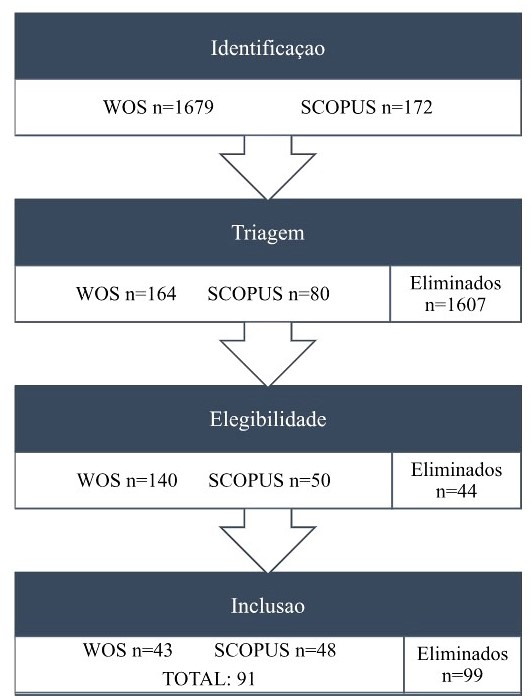
\includegraphics[width=0.6\linewidth]{Fig1.jpg}
    \caption{Diagrama de fluxo do processo seguido.}
    \source{Elaboração própria baseada no Método PRISMA.}
    \label{fig1}
\end{figure}

Como critério de inclusão utilizou-se apenas o tipo de documento, sendo selecionados apenas artigos publicados em periódicos, excluindo editoriais, cartas, capítulos de livros e outros tipos de publicações. Não foram utilizados critérios relacionados à data de publicação, à área do conhecimento, ao país ou ao idioma.

Em seguida, para a análise do material e representação dos dados, foram utilizados os programas \textit{VosViewer} \cite{van_eck_text_2011} e \textit{RStudio}, versão R-4.2.3, \cite{r_core_team_r:_2016}, ambas ferramentas de programação que permitem a análise de dados relacionados à bibliometria.

No \textit{RStudio} foi utilizado o pacote \textit{bibliometrix} (versão 4.0.0), que dá acesso ao \textit{biblioshiny}, uma extensão web que torna a utilização do \textit{bibliometrix} mais dinâmica, permitindo a interpretação e a criação de representações gráficas \cite{aria_bibliometrix_2017}. Por meio dos programas foi possível identificar periódicos, autores, instituições e países mais proeminentes na área de pesquisa, bem como as principais redes colaborativas de pesquisa entre autores, redes de cocitação e principais áreas temáticas no campo.

Com relação ao gráfico de evolução temática, ele é estruturado no \textit{biblioshiny} tendo como base a densidade das palavras-chave dos artigos ao longo de todo o período analisado. O \textit{software} estabelece então um gráfico baseado em centralidade do tema (eixo vertical), ou seja, o quanto aquele tema está sendo discutido como um todo na amostra, e na densidade do tema (eixo horizontal) quantas vezes ele se repete em toda a amostra ao longo do período. Em outras palavras, a centralidade avalia a importância do tema na área, enquanto a densidade reflete o seu nível de desenvolvimento \cite{shi_mapping_2021}.

O \textit{software} gera então um gráfico com quatro quadrantes que divide os temas em 1) fundamentais ou básicos: temas bastante pesquisados e já estabelecidos na área, 2) emergentes ou em declínio: temas recentes que podem estar em avanço ou declinando, 3) temas de nicho: temas muito específicos ou subtópicos na área, e 4) temas motores: os quais podem indicar tópicos de tendência e a provável direção de uma futura agenda de pesquisa na área \cite{ortiz-rojo_empreendedorismo_2023}.


\section{Resultados}

\subsection{Crescimento da pesquisa na área, principais periódicos, autores e instituições envolvidas}

A busca nas bases resultou em 91 documentos publicados em 56 fontes. Conforme mostra o gráfico da \Cref{fig2}, esses documentos estão distribuídos ao longo de 28 anos com o primeiro registro datado de 1995, a média anual de publicação é de 6,91.

Analisando o gráfico da \Cref{fig2}, vemos que as publicações na área passam por algumas oscilações e que essa produção só alcança crescimento mais substancial a partir de 2018, com pico em 2022. Vale ressaltar que a pesquisa foi feita em maio de 2023, assim, é possível que a pesquisa continue num crescente, especialmente tendo em vista que nesse momento do ano as publicações já se igualam a todo o ano de 2018.

\begin{figure}[h!]
    \centering
    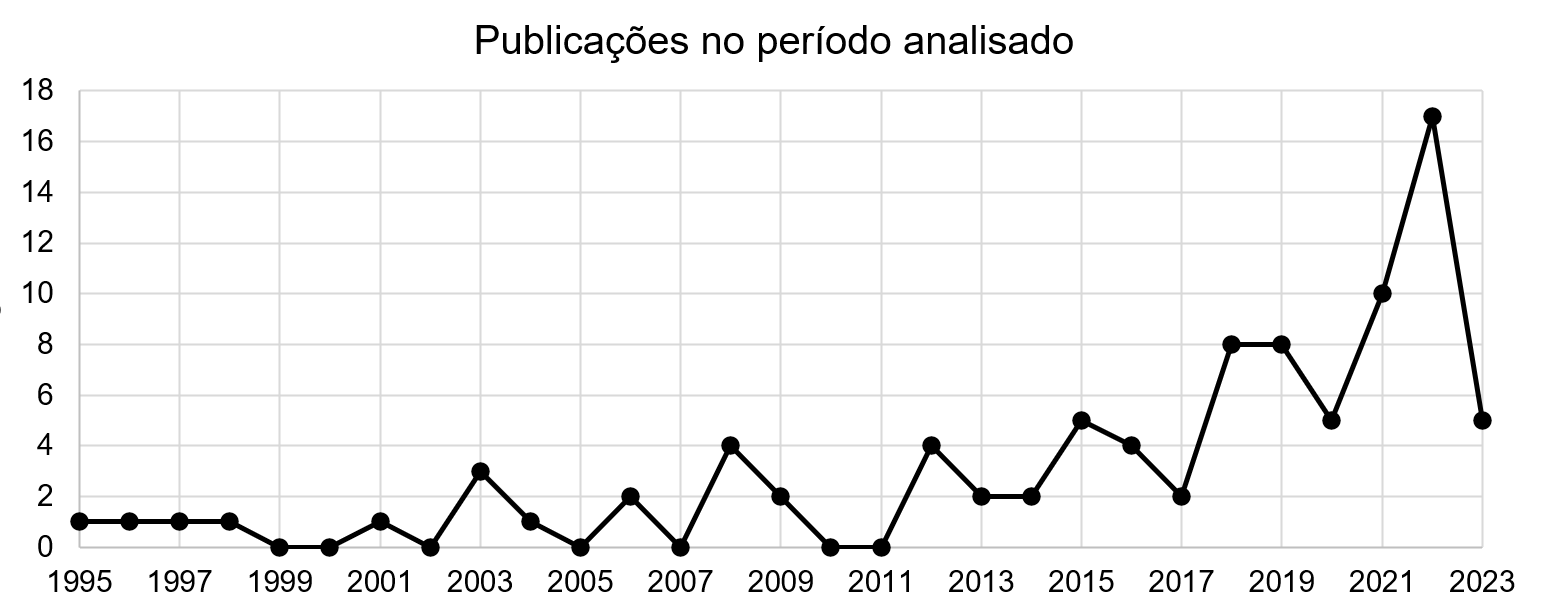
\includegraphics[width=0.8\linewidth]{Fig2.png}
    \caption{Produção anual na área pesquisada de 1995 a 2023.}
    \label{fig2}
    \source{Elaboração própria.}
\end{figure}

Em relação aos periódicos de maior relevância, das 56 fontes encontradas foram selecionadas as 10 com o maior número de publicações no tema, as quais detém juntas cerca de 44\% (40) do total de artigos encontrados na pesquisa, como mostra a \Cref{tab1}. Foi elencado também o fator de impacto de cada um dos periódicos mencionados, que leva em consideração a média de citações recebidas por artigo publicado em um periódico considerando os dois anos anteriores \cite{silva_associacao_2018,agarwal_bibliometrics:_2016}.

Ter conhecimento de quais periódicos possuem mais impacto na área, assim como seu escopo, direcionará o olhar do pesquisador ou do docente em atuação para publicações mais bem consolidadas, o que pode gerar pesquisas fundamentadas em um referencial sólido, além de estimular o desenvolvimento de inovações ou a ampliação de propostas já previamente testadas \cite{pereira_ensino_2020}.

\begin{table}[h!]
\centering
\begin{threeparttable}
\caption{Os 10 principais periódicos de acordo com o volume de publicações no tema, seu índice H e fator de impacto.}
\label{tab1}
\begin{tabular}{l l l}
\toprule
 Periódicos & N° Artigos & Fator de Impacto \\
 \midrule
\rowcolor[HTML]{EFEFEF}American Biology Teacher & 9 & 0.485 \\
Biochemistry and Molecular Biology Education & 5 & 1.369 \\
\rowcolor[HTML]{EFEFEF}Journal of Science Education and Technology & 5 & 3.419 \\
Advances in Physiology Education & 4 & 2.396 \\
\rowcolor[HTML]{EFEFEF}Journal of Chemical Education & 4 & 3.208 \\
British Journal of Educational Technology & 3 & 5.268 \\
\rowcolor[HTML]{EFEFEF}Cbe-Life Sciences Education & 3 & 3.955 \\
Frontiers in Education & 3 & 2.320 \\
\rowcolor[HTML]{EFEFEF}ChemComm (Chemical Communications) & 2 & 6.065 \\
Education Sciences & 2 & 2.920 \\
\bottomrule
\end{tabular}
\source{Elaboração própria.}
\end{threeparttable}
\end{table}

Assim, se só considerarmos o número de publicações, a revista \textit{American Biology Teacher} seria a mais relevante na área. Contudo, ao levarmos em consideração o fator de impacto das revistas, os dois periódicos que se destacam são \textit{ChemComm} (\textit{Chemical Communications}) e \textit{British Journal of Educational Technology}. É comum no ramo da educação que revistas de ensino de ciências abarquem publicações de todas as áreas relacionadas às ciências da natureza. A primeira revista, no entanto, é focada na área do ensino de química, a segunda é uma revista com temas mais gerais e foco no uso de tecnologias educacionais.

Quanto aos autores, foram encontrados 362, sendo a média de autores por documento de número quatro. Assim, apenas 9 são autores de documentos de autoria única. Os 10 pesquisadores com o maior número de artigos publicados estão listados na \Cref{fig3}. Ao analisá-la pode-se observar que não há autores com elevado número de publicações no período. Muitos, inclusive, são coautores de produções mostradas. Nove dos dez autores que mais publicaram na área possuem artigos bastante recentes, publicados a partir de 2017.

\begin{figure}[h!]
    \centering
    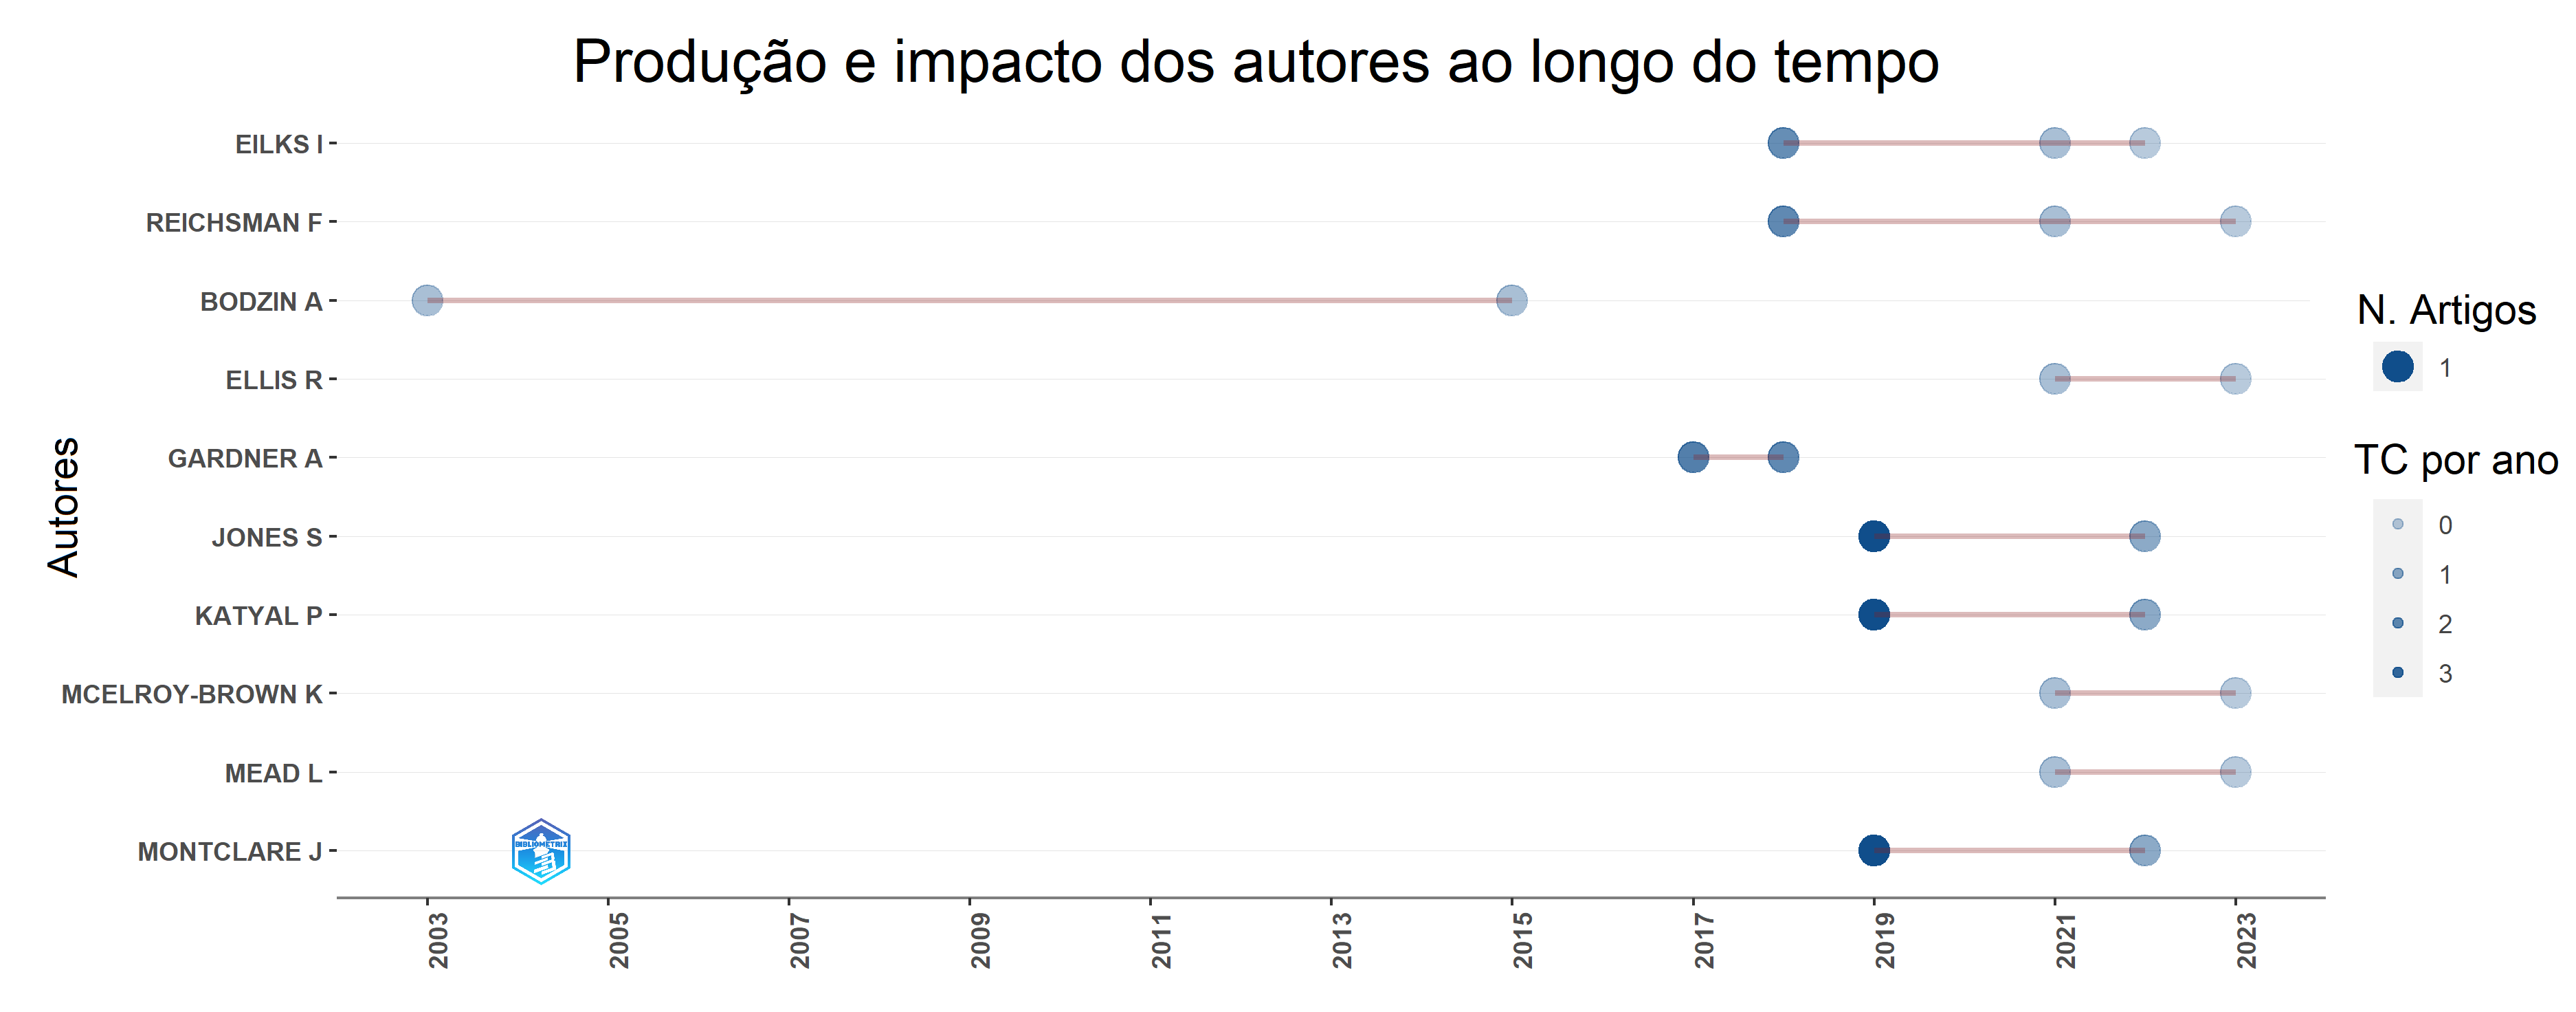
\includegraphics[width=0.9\linewidth]{Fig3.png}
    \caption{Produção dos 10 autores que mais publicaram ao longo do período analisado. Os círculos indicam o volume de publicações e a coloração o impacto, quanto mais escuro, maior o número de citações.}
    \label{fig3}
    \source{Obtido por meio da inserção de dados da pesquisa no Bibliometrix.}
\end{figure}

Com relação às afiliações com maior número de publicações, a Universidade Northwestern e a Universidade da Califórnia foram as mais representadas, com nove publicações cada uma. Vale ressaltar que a Universidade de Brasília figura entre as que mais publicaram, com cinco artigos sobre o tema. Os países com a maior produção no período analisado são Estados Unidos e Indonésia com 39 e 9 publicações respectivamente; em seguida tem-se a Brasil (7), China (6), Alemanha (5), Austrália (2), Suíça (2), Reino Unido (2), Argentina (1) e Chile (1). A \Cref{fig4} contempla estes e outros países com ao menos uma publicação na área no período analisado.

\begin{figure}[h!]
    \centering
    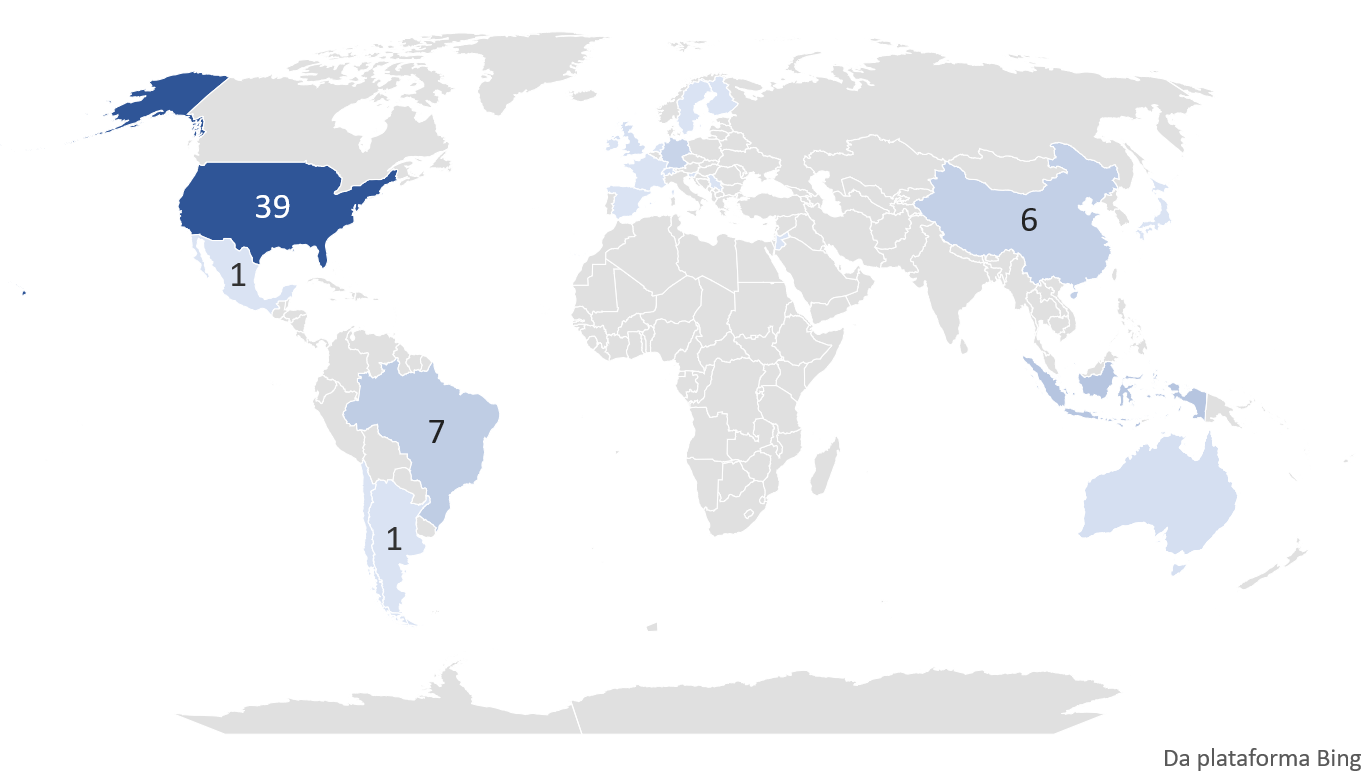
\includegraphics[width=0.8\linewidth]{Fig4.png}
    \caption{Países que publicaram ao menos 1 artigo ao longo do período analisado estão destacados em tons de azul.}
    \label{fig4}
    \source{Elaboração própria.}
\end{figure}

\subsection{Redes de colaboração e cocitação}

A \Cref{fig5} apresenta as redes de colaboração entre os 50 autores com ao menos duas colaborações entre si, considerando todos os anos de produção. Os critérios da busca revelaram apenas 47 autores.

Analisando o maior \textit{cluster} ilustrado pela \Cref{fig5}, o vermelho, temos o total de sete autores em colaboração. Três deles são da Concord Consortium, uma organização sem fins lucrativos, localizada em Massachussets nos Estados Unidos, e os demais são da Universidade de Michigan, também nos Estados Unidos. A publicação mais recente feita por essa rede de autores aborda o ensino de evolução por meio do desenvolvimento de um conjunto de lições interativas, \textit{on-line} e de livre acesso que se concentram na evolução das ervilhas-de-cheiro a partir de seus ancestrais com sabor de amido \cite{ellis_connected_2023}.

As lições propostas pelo artigo estão vinculadas ao \textit{Next Generation Science Standards}, ou seja, integram conceitos em várias escalas e foram projetadas para serem usadas em uma ordem flexível, com suporte fornecido aos professores sobre como escolher uma sequência que atenda às necessidades dos alunos \cite{ellis_connected_2023}. Esse nível de adaptação e personalização do ensino, embora ainda não seja individual, aproxima mais o conteúdo do contexto dos docentes e do alunado, e já mostra um esforço consistente com a necessidade constante de adaptar o ensino aos diferentes perfis de estudantes.

Com relação ao \textit{cluster} verde, apenas um autor é do \textit{Institute of Math and Science for Young Women}, os demais são da Escola de Engenharia Tandon da Universidade de Nova York, nos Estados Unidos. A publicação mais recente do grupo de pesquisa aborda a efetividade de uma proposta de ensino baseada em jogos, para ensinar o dogma central da biologia molecular, com auxílio do \textit{Kahoot} \cite{jones_kahoot!_2019}. Como conclusão os autores apontam que a ferramenta de avaliação gamificada pode ajudar os alunos a aprenderem o tópico, envolvendo-os ativamente de forma divertida e empolgante. Devido às suas acessibilidade e boa usabilidade, o \textit{Kahoot} pode ser uma boa ferramenta para professores apresentarem um sistema de resposta a testes divertido e exclusivo, mais atraente para os alunos em comparação com os sistemas convencionais \cite{licorish_students_2018}.

\begin{figure}[h!]
    \centering
    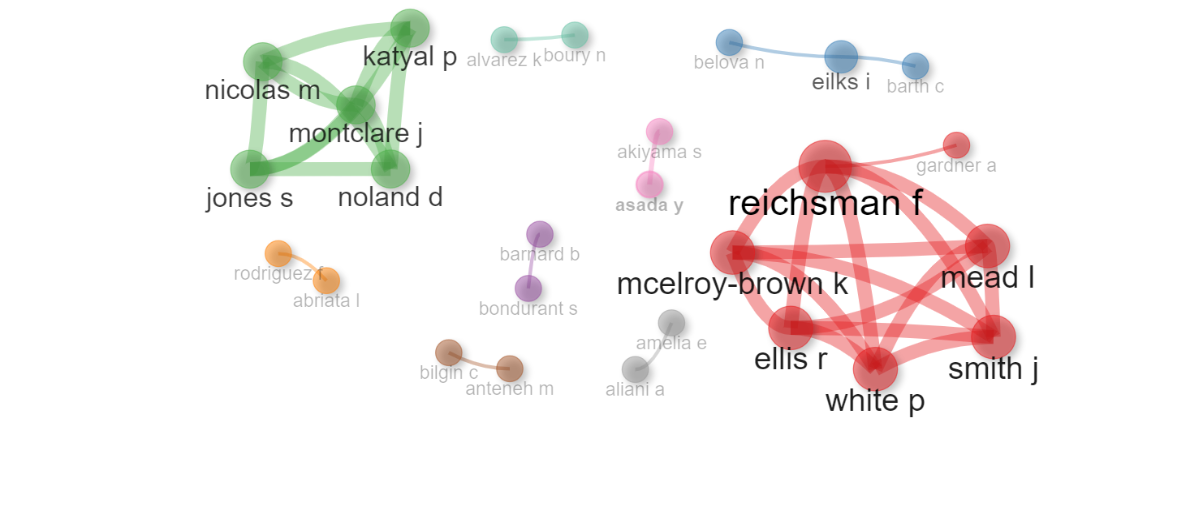
\includegraphics[width=0.8\linewidth]{Fig5.png}
    \caption{Rede de colaboração entre os autores mais relevantes na área.}
    \label{fig5}
    \source{Obtido por meio da inserção de dados da pesquisa no Bibliometrix.}
\end{figure}


Ainda tratando sobre as redes de colaboração, foram identificados três tipos de redes nas análises. Primeiramente, aquelas envolvendo pesquisadores de uma mesma instituição, como por exemplo o trabalho de \textcite{nurhayati_application_2022}, o qual focou em um aplicativo móvel de realidade aumentada, cujos autores são todos pertencentes à Universidade Negeri Jakarta da Indonésia. Em segundo lugar, há redes de colaboração interinstitucionais, mas intranacionais, ou seja, são redes criadas entre investigadores de instituições diferentes, mas do mesmo território nacional, como, por exemplo, o artigo de \textcite{chuang_using_2023} sobre Realidade Virtual, escrito por autores do Nantou Hospital e da Universidade Médica de Chung Shan em Taiwan. Finalmente, existem também redes de colaboração internacional, embora em menor escala, as quais contam com a participação de pesquisadores de diferentes países ou mesmo continentes. Um exemplo deste último tipo de rede é o documento de \textcite{dewi_development_2018} sobre contação de histórias, escrito por autores de instituições educacionais da Indonésia e da Malásia. Cabe destacar que a última rede é a que aparece com menor frequência, tendo em vista o fato de que o percentual de colaboração internacional de todas as pesquisas é de apenas 9,8\%.

A \Cref{fig6}, por sua vez, indica as redes de cocitação na área. O \textit{cluster} verde apresenta documentos oficiais americanos sendo citados, como o \textit{Design-Based Research}, o qual apresentava em 2003 um paradigma emergente para a pesquisa educacional, proposto por um coletivo de pesquisadores \cite{the_design-based_research_collective_design-based_2003}; e, o documento do \textit{National Research Council} que apresenta uma estrutura de práticas, conceitos transversais e ideias centrais para o ensino de Ciências e Biologia no ensino fundamental e médio \cite{national_research_council_framework_2012}. Parece um \textit{cluster} dedicado a nortear pesquisas que propõem novos métodos de ensino de biologia em todos os anos da educação básica.

\begin{figure}
    \centering
    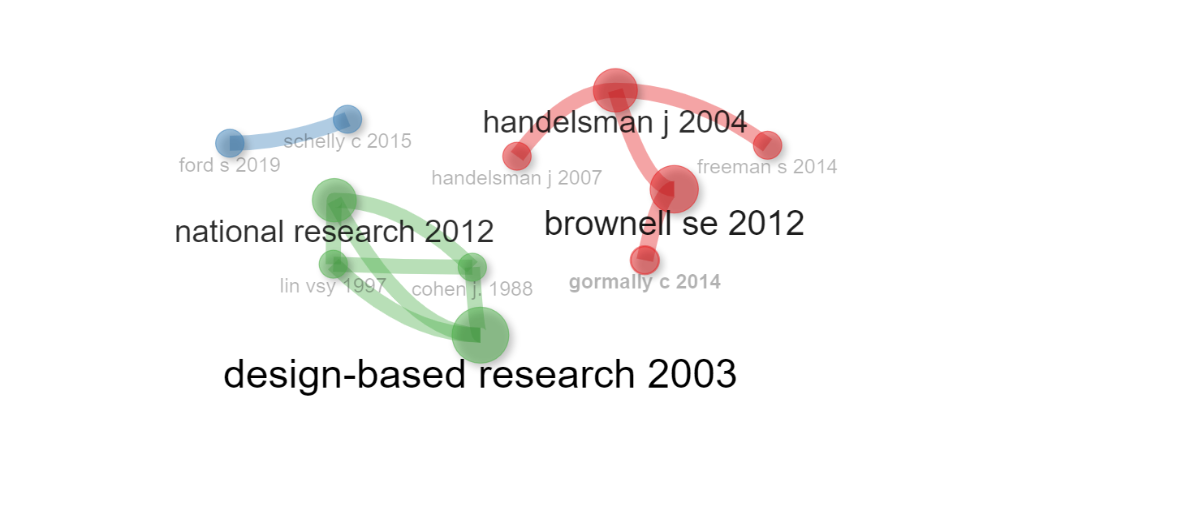
\includegraphics[width=0.8\linewidth]{Fig6.png}
    \caption{Redes de cocitação. Foram considerados os 50 documentos mais citados nas referências da amostra desta pesquisa.}
    \label{fig6}
    \source{Obtido por meio da inserção de dados da pesquisa no Bibliometrix.}
\end{figure}

Ao analisar a rede representada em vermelho, dois documentos se destacam. O artigo de \textcite{handelsman_scientific_2004} apresenta o ensino científico como uma base para o ensino eficaz, aplicável, real e emancipador, promovendo o aprendizado ativo, o pensamento crítico e o desenvolvimento da alfabetização científica.

O artigo de \textcite{brownell_undergraduate_2012}, por sua vez, destaca a necessidade de uma remodelagem nas aulas práticas aplicadas em laboratório nas aulas de biologia, pontuando que em vez de uma estrutura tradicional, muitas vezes descrita como "livro de receitas", deveriam ser projetadas experiências autênticas baseadas em pesquisa. Os autores comparam um curso de laboratório do tipo livro de receitas com um curso de laboratório baseado em pesquisa e constataram que os alunos do laboratório baseado em pesquisa tinham atitudes mais positivas em relação à pesquisa autêntica, maior autoconfiança em tarefas relacionadas ao laboratório e maior interesse em realizar pesquisas futuras em comparação com os alunos do curso de laboratório de livros de receitas.

A partir da breve descrição desses documentos, pode-se inferir que a rede possui um interesse em evidências empíricas que apoiam as recomendações para a incorporação de componentes de pesquisa mais autênticos no ensino de ciências e biologia. Também é intuito dos autores promover um ensino científico alinhado às expectativas do presente século.

\subsection{Evolução temática das pesquisas na área}

A \Cref{fig7} indica o resultado da análise da evolução temática tendo como base as palavras-chave mais frequentes ao longo de todo o tempo de amostragem. É possível observar que educação a distância era um tema emergente, mas já está migrando para um tema básico, ou seja, um tema fundamental na pesquisa que envolve ensino de biologia e disciplinas na área de ciências naturais atualmente.

\begin{figure}[h!]
    \centering
    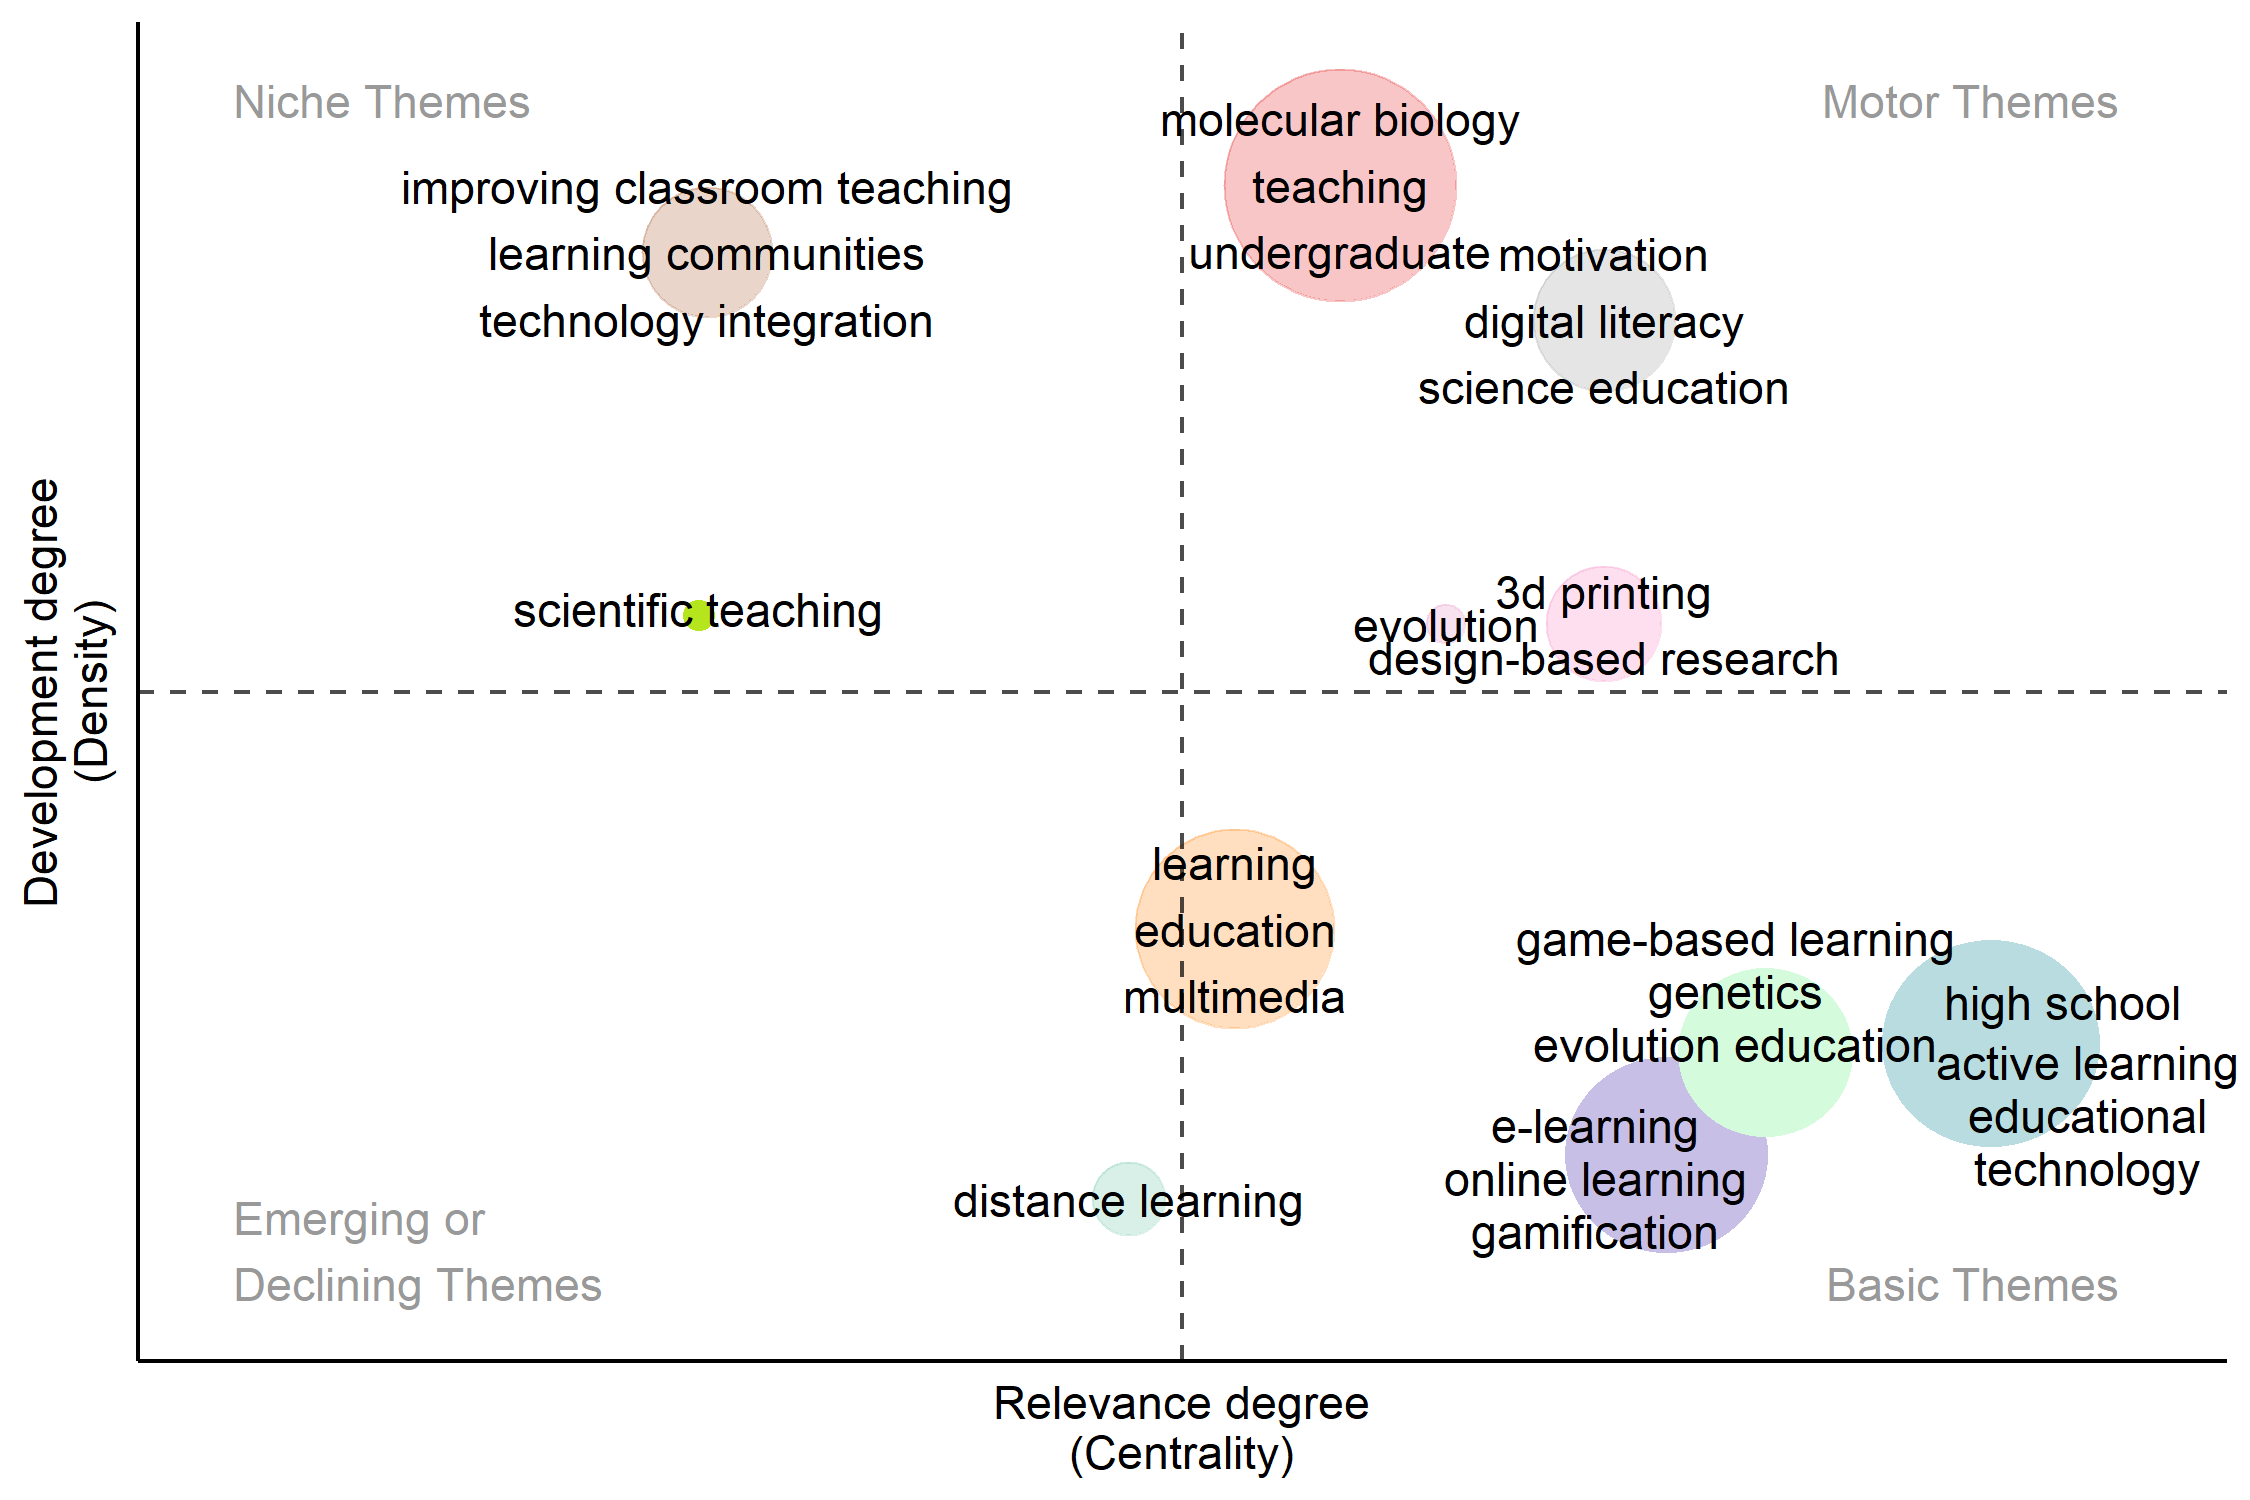
\includegraphics[width=0.8\linewidth]{Fig7.png}
    \caption{Evolução temática indicando temas de nicho, emergentes, motores e básicos na área pesquisada.}
    \label{fig7}
    \source{Obtido por meio da inserção de dados da pesquisa no Bibliometrix.}
\end{figure}

Os temas de nicho, por sua vez, referem-se a tópicos específicos ou especializados que têm um escopo ou apelo limitado dentro do domínio de pesquisa mais amplo. Nesse sentido, comunidades de aprendizado e integração da tecnologia parecem ser um subcampo dentro da área de interesse maior. Entretanto, temas de nicho também podem surgir de áreas emergentes de pesquisa, nesse caso, a educação científica encaixa-se nesse aspecto do quadrante.
Com relação aos temas básicos, estes abrangem ideias centrais ou metodologias consideradas fundamentais no campo. Os temas básicos geralmente são atemporais e no caso da presente pesquisa, gamificação, aprendizagem ativa e \textit{e-learning} aparecem nesse quadrante. Além destes, os conteúdos de evolução e genética são os mais presentes nas pesquisas da amostra.

Por fim, os temas motores, são tópicos que podem auxiliar a predizer a direção de pesquisas futuras e moldar a trajetória geral da área. Em nosso caso, os conteúdos de biologia molecular e evolução estão em alta, mantendo o padrão similar em relação aos conteúdos básicos. Os termos motivação, literacia ou alfabetização digital e educação científica surgem também como temas motores. Além destes, mais abaixo no mesmo quadrante, próximo aos temas básicos estão os termos \textit{design-based research} e impressão 3D.

\section{Discussão}
O aumento acentuado nas pesquisas na área da tecnologia educacional, em especial a partir do ano de 2020, é apresentado na literatura como consequência do contexto pandêmico vivenciado nos últimos tempos \cite{ibanez_educacion_2020}. \textcite{garcia_percepcao_2022} afirmam que mesmo com várias atividades sendo interrompidas, no caso do ensino, muitas foram readaptadas para o formato remoto e prosseguiram levantando dados sobre o novo cenário da educação.

Mesmo antes da pandemia, já havia indicações claras de aumento no uso da tecnologia em sala de aula, mas o contexto pandêmico promoveu uma acentuada elevação no número de pesquisas envolvendo o desenvolvimento e avaliação de recursos de ensino tecnológicos, tendo em vista a necessidade iminente de progredir com os anos letivos ao mesmo tempo em que se mantinha o distanciamento social, como revela a literatura \cite{ibanez_educacion_2020}. Tal fato justifica a manutenção das pesquisas em alta no gráfico indicado pela \Cref{fig2}.

Com relação aos países que mais publicam, a presença do Brasil entre os 10 países mais proeminentes na área demonstra que esforços estão sendo empregados para a melhoria do letramento científico e tecnológico mesmo em países em desenvolvimento. Entretanto, muito ainda se discute sobre o distanciamento entre o ensino e aprendizagem de ciências naturais, e mais especificamente na biologia, e o que é vivenciado no cotidiano dos alunos, um problema presente desde a formação de professores até a educação básica no Brasil \cite{moura_biologia/genetica:_2013,pereira_estrategias_2020}.

É válido ressaltar que tal fato também se aplica a países com extensa produção. Nos Estados Unidos, por exemplo, as pesquisas observam grande defasagem no ensino de genética e áreas correlatas \cite{barros_o_2017}. Isso demonstra que, embora exista um crescente volume de trabalhos direcionados à melhoria da educação na área das ciências naturais, poucos ultrapassam as paredes da academia, o que acentua e perpetua a lacuna entre pesquisa e prática \cite{lawlor_approaches_2019}.

Outro dado relevante são as redes de colaboração. O estudo dessas redes pode fornecer valiosos indicadores que propiciam o entendimento da construção do conhecimento de uma área de interesse \cite{hilario_2020}. Com relação à rede de colaboração indicada pelo \textit{cluster} vermelho (\Cref{fig5}), é possível identificar um direcionamento para a personalização no ensino. As salas de aula modernas estão mais diversificadas do que nunca. Contudo, os métodos de ensino ainda são empregados de maneira generalista com o percurso padronizado, apesar de facilmente identificarmos que a aprendizagem é uma viagem pessoal. Assim, é urgente e necessário empreender esforços no sentido de promover a adaptação das experiências de aprendizagem às necessidades únicas de cada aluno \cite{santos_aplicacao_2020}.

Ademais, com os percursos profissionais cada vez mais personalizados, as nossas salas de aula precisam estar mais alinhadas à essa expectativa. Um dos benefícios ocultos da aprendizagem personalizada é a sua capacidade de cultivar uma mentalidade de aprendizagem autônoma, tendo em vista que, nesse modelo, os estudantes têm a liberdade de aprenderem em um ritmo adequado ao seu nível pessoal de capacidade, reduzindo a necessidade de "acompanhar a aula" obrigatoriamente no tempo dos demais colegas \cite{santos_aplicacao_2020}. Este é um dos benefícios claros do uso de RED no ensino em todos os níveis.

No \textit{cluster} verde a gamificação aparece em destaque. A literatura aponta que elementos gamificados, os quais integram vibração, música leve e competição, são úteis para manter os alunos atentos durante todo o jogo, e como resultado, podem averiguar o próprio conhecimento em tempo real, permitindo correções pontuais por parte do docente \cite{lin_kahoot!_2018}. Ao acentuar a motivação e o envolvimento dos alunos, a proposta ajuda-os a aprender ativamente até mesmo as matérias consideradas mais difíceis, tais como são consideradas as disciplinas nas áreas das ciências naturais \cite{jones_kahoot!_2019}.

Além das redes de colaboração, a análise das redes de cocitação também é relevante, tendo em vista o fato de que estas possibilitam a identificação de linhas de pesquisa consolidadas, assim como de autores e estudos de alta relevância para a área \cite{castanha_estudos_2020}. A respeito dos documentos mais citados no \textit{cluster} verde, é importante mencionar que a pesquisa baseada em design deve fundamentar a maior parte dos recursos tecnológicos desenvolvidos para fins educativos. Isso porque ela combina a pesquisa educacional empírica com o design de ambientes de aprendizagem orientado pela teoria, além de ser uma metodologia importante para entender como e porque as inovações educacionais funcionam na prática \cite{kennedy-clark_reflection:_2015}.

Com relação ao documento do \textit{National Research Council}, ao explorar documentos de pesquisa e políticas de educação científica, foi possível que os autores sintetizassem as visões atuais da filosofia da ciência e propusessem uma distinção entre o processo científico e o resultado objetivo da investigação científica, estabelecendo metas mais precisas e propondo métodos de ensino mais coerentes com o que é esperado dos estudantes \cite{keller_framework_2012}.

O \textit{cluster} vermelho, por sua vez, aborda o ensino científico, apoiado por RED, com maior profundidade. O ensino científico incentiva os alunos a um aprendizado contínuo, a serem participantes ativos em seu aprendizado por meio de atividades baseadas em investigação. Os alunos são estimulados a desenvolver o pensamento crítico por meio da análise e avaliação de informações, identificando preconceitos, fazendo conexões entre conceitos e desenvolvendo habilidades de raciocínio lógico \cite{american_association_for_the_advancement_of_science_vision_2011}.

O ensino científico também enfatiza a importância de basear as conclusões e explicações em evidências. Por fim, os estudantes são incentivados a trabalhar em grupos, participar de discussões e compartilhar suas descobertas \cite{couch_scientific_2015}. Dessa forma, ao aplicar o ensino científico, tendo como apoio RED, os alunos aprendem a aplicar seus conhecimentos a situações do mundo real e a fazer conexões entre diferentes disciplinas científicas, proposta que vai além do livro didático e promove um ambiente em que os alunos são incentivados a propor novas ideias, testar hipóteses e pensar criticamente sobre conceitos científicos \cite{couch_scientific_2015}.

Embora a análise das redes de colaboração e cocitação ofereça uma visão dos temas mais frequentes na área de interesse da presente pesquisa, é essencial verificar se esses temas estão presentes na pesquisa atual ou se fazem parte de propostas já saturadas e em declínio. Afinal, os temas emergentes e de destaque podem indicar caminhos para inovação e direcionar novas propostas de pesquisa, visto que ajudam os pesquisadores e profissionais a identificar tendências, mudanças de foco e áreas que exigem maior exploração ou investigação. Nesse sentido, a \Cref{fig7} indica o resultado da análise da evolução temática tendo como base as palavras-chave mais frequentes ao longo de todo o tempo de amostragem.

Com relação à evolução temática, é possível observar que educação à distância era um tema emergente, mas já está migrando para um tema básico, ou seja, um tema fundamental na pesquisa que envolve RED, ensino de biologia e disciplinas na área de ciências naturais. Sem dúvida a educação à distância não surgiu recentemente, na área das ciências naturais, há diversas pesquisas indicando recursos utilizados para substituir ferramentas como microscópios ou mesmo alternativas viáveis para substituir o formato convencional de laboratório prático \cite{winkelmann_development_2017}.

Entretanto, tendo em vista o contexto de pandemia, houve um natural aumento no número de publicações considerando o contexto remoto implementado. Assim, muitos pesquisadores passaram a publicar sobre o assunto revelando que a implementação emergencial da educação à distância ou do ensino na modalidade remota gerou diversos desafios, partindo desde questões como a presença de estudantes em intercâmbio e as dificuldades no processo avaliativo à distância, até questões relacionadas ao impacto potencial do distanciamento social na saúde mental dos estudantes e das equipes de apoio técnico-pedagógico \cite{sahu_closure_2020}. Foco também muito comum no mesmo período foi a análise de abordagens de ensino experimentadas na pandemia, revelando como e quão bem elas funcionaram \cite{holme_introduction_2020}.

Com relação aos temas de nicho, um dos tópicos que surgiu de uma área emergente de pesquisa, foi a educação científica, já previamente discutida nas redes de cocitação. Os fundamentos do ensino científico têm sido um dos principais percursos norteadores na produção de recursos educativos digitais e, portanto, é possível que migrem deste quadrante para o quadrante de temas básicos \cite{handelsman_scientific_2004,couch_scientific_2015}.

Com relação ao quadrante de temas básicos, a gamificação e a aprendizagem ativa aparecem com mais proximidade ao centro de relevância do gráfico. Estas são duas abordagens educacionais que ganharam muita atenção nos últimos anos devido ao seu potencial para aumentar o envolvimento dos alunos e melhorar os resultados da aprendizagem. Enquanto a gamificação se refere ao uso de elementos e princípios de design de jogos em contextos que não são de jogos, a aprendizagem ativa envolve a promoção da participação, interação e envolvimento do aluno no processo de aprendizagem. Embora sejam conceitos distintos, há características que se sobrepõem entre a gamificação e a aprendizagem ativa que podem ser mutuamente benéficas em ambientes educacionais.

A gamificação pode ser aplicada a metodologias de aprendizagem ativa para criar uma experiência de aprendizagem mais imersiva e interativa \cite{jones_kahoot!_2019}. Ao incorporar elementos de jogos ela promove a motivação intrínseca e torna o aprendizado mais agradável, além de envolver os alunos ativamente no processo de aprendizagem \cite{subhash_gamified_2018}. Vários estudos exploraram a relação entre a gamificação e a aprendizagem ativa, destacando seus benefícios e eficácia em contextos educacionais \cite{murillo-zamorano_gamification_2021,seaborn_gamification_2015,subhash_gamified_2018}.

Ainda neste quadrante, com relação aos conteúdos, evolução e genética foram os mais frequentemente encontrados nas pesquisas. Na Biologia estes são os conteúdos considerados mais desafiadores. Pesquisas apontam que a grande demanda de elementos conceituais abstratos e em nível molecular, a incompreensão de cálculos, assim como as dificuldades em fazer associações interdisciplinares, são os principais obstáculos apontados no aprendizado de genética \cite{fabricio_compreensao_2006,catarinacho_o_2011}.

No caso da evolução, crenças pessoais, a impossibilidade de observação dos eventos de forma concreta, tendo em vista a premissa do tempo, a incompreensão com relação à natureza da ciência e a dificuldade de compreensão da linguagem e terminologia dos conceitos básicos relacionados ao tema, são apontados como principais motivos pelos quais os estudantes possuem dificuldade de compreensão da disciplina \cite{gregory_understanding_2009,sinatra_intentions_2003,rutledge_evolutionary_2000}.

Outro termo presente é a alfabetização digital que se refere à capacidade de navegar, avaliar, compreender e criar informações de forma eficaz usando tecnologias digitais. Ela engloba uma série de habilidades, inclusive envolver-se em um comportamento \textit{on-line} responsável e ético \cite{livingstone_balancing_2010}. A alfabetização digital tornou-se um tópico importante nos últimos anos devido a vários fatores. Primeiro, o avanço tecnológico crescente torna essencial a habilidade de manipular e interagir com recursos e plataformas \cite{koltay_media_2011}. Em segundo lugar, a proficiência em ferramentas e tecnologias digitais é cada vez mais exigida em várias funções de trabalho, e as instituições educacionais estão integrando a alfabetização digital em seus currículos.

Além de uma quantidade sem precedentes de informações, a era digital trouxe também a proliferação de desinformação e notícias falsas. A alfabetização digital ajuda as pessoas a desenvolver habilidades para avaliar e verificar criticamente as informações que encontram \textit{on-line}, permitindo que tomem decisões informadas e evitem ser vítimas de desinformação. Tais aspectos se relacionam diretamente com uma educação científica de qualidade.

Além disso, em uma sociedade cada vez mais digital, as pessoas que não possuem habilidades de alfabetização digital podem enfrentar barreiras no acesso a informações, recursos, educação, oportunidades de trabalho e participação cívica \cite{warschauer_new_2010}. Eliminar a lacuna de alfabetização digital é fundamental para promover a igualdade de oportunidades e reduzir a exclusão digital.

A impressão de modelos 3D, frequentemente utilizados na produção de recursos para ensino de conteúdos abstratos ou microscópicos, também surge como tema motor. Isso se deve provavelmente porque a impressão 3D proporciona aos alunos uma experiência de aprendizado prático, na qual eles podem projetar e criar objetos físicos \cite{pernaa_systematic_2020}. Isso permite que eles transformem suas ideias em protótipos tangíveis, estimulando a criatividade, a resolução de problemas e as habilidades de pensamento crítico.

Propostas assim também permitem a integração de várias disciplinas, como design, engenharia, matemática e ciência da computação, ou seja, estão alinhadas com as proposições atuais de promover a interdisciplinaridade no ensino de ciências e a aproximação dos estudantes da busca por soluções a problemas reais e cotidianos \cite{hansen_exploring_2020}. Assim, a introdução da impressão 3D na educação ajuda os alunos a conectar o aprendizado em sala de aula a aplicações no mundo real, preparando-os para futuras carreiras em campos que utilizam essa tecnologia \cite{pernaa_systematic_2020}.

Na mesma posição no quadrante, surge o \textit{design-based research}, o qual se mantém como tema motor, por ainda ser bastante aplicado no desenvolvimento de recursos educativos digitais, mas se posiciona bem próximo do quadrante de temas básicos, por já se estabelecer como metodologia considerada essencial para a compreensão e realização de pesquisas no campo em questão.

\section{Considerações finais}

O presente estudo bibliométrico mostra um aumento da produção científica sobre RED na área das Ciências Naturais nos últimos anos, com um pico no ano 2022, o que poderia indicar que o "regresso à normalidade" após a pandemia consolidou algumas das mudanças no uso da tecnologia e dos diversos materiais didáticos digitais que os professores utilizaram, em tempo recorde, durante o confinamento \cite{rodriguez_materiales_2020}.

Da mesma forma, a análise tanto dos artigos mais citados como dos temas emergentes prevê uma mudança no Ensino Médio a favor da aplicação de propostas focadas na aprendizagem ativa, no desenvolvimento do pensamento crítico, da literacia científica, além de apontar para uma necessidade iminente de se trabalhar com base em experiências autênticas, baseadas na investigação, em que os alunos são os principais protagonistas dos processos de ensino e aprendizagem. Estas questões implicam, por um lado, a necessidade de avaliar se os materiais didáticos digitais que estão sendo utilizados nas salas de aula cumprem as funções que se pretendem alcançar na área das Ciências Naturais (reforço visual, modelos 3D, interatividade, movimento, aumento da motivação ou participação, etc.) e, por outro lado, avaliar que mecanismos a administração educativa estão sendo postos em prática para preencher algumas das lacunas que encontramos na implementação de RED nas salas de aula atualmente, tais como limitações tecnológicas, necessidade de formação de professores ou falta de tempo \cite{vidal_esteve_uso_2019}.

Quanto às limitações deste trabalho, é possível apontar para a utilização de somente duas bases de dados, que apesar de possuírem reconhecido prestígio, não permitem incorporar à análise trabalhos que tenham sido publicados em periódicos que não estejam indexados nelas. Além disso, a altimetria não foi utilizada na análise bibliométrica para saber o peso dos autores nas redes colaborativas. E, por fim, dada a extensão da proposta, não foi incorporada neste trabalho a análise de conteúdo dos artigos, o que, sem dúvida, nos permitiria aprofundar nas contribuições que os RED têm oferecido nos processos de ensino e aprendizagem na área de ciências naturais.

Estas três questões são levantadas como linhas de investigação prospectivas ou futuras, juntamente com a análise por territórios, que permitirão confrontar os resultados com base nas políticas levadas a cabo pela Administração educativa.

\section{Agradecimentos}

Este artigo é parte de um projeto de pesquisa de pós-doutorado e também está vinculado ao projeto intitulado “Materiais didáticos digitais na educação secundária obrigatória: análises e propostas para seu uso escolar e sociofamiliar” (PID2022-1373660B-100), aprovado à convocação em 2022 para “Projetos de Geração de Conhecimento” do Ministério da Ciência e Inovação do Governo da Espanha. Agradecemos aos dirigentes e colaboradores do Instituto Federal de Educação, Ciência e Tecnologia de Brasília / Brasil, assim como ao Departamento de Didática e Organização Escolar da Universidade de Valência / Espanha.


\printbibliography\label{sec-bib}
% if the text is not in Portuguese, it might be necessary to use the code below instead to print the correct ABNT abbreviations [s.n.], [s.l.]
%\begin{portuguese}
%\printbibliography[title={Bibliography}]
%\end{portuguese}


%full list: conceptualization,datacuration,formalanalysis,funding,investigation,methodology,projadm,resources,software,supervision,validation,visualization,writing,review
\begin{contributors}[sec-contributors]
\authorcontribution{Mayara Lustosa de Oliveira Barbosa}[conceptualization,formalanalysis,projadm,supervision,validation,visualization,writing,review]
\authorcontribution{Diana Marín-Suelves}[datacuration,funding,methodology,supervision,validation,visualization,writing,review]
\authorcontribution{Cecilia V. Becerra-Brito}[investigation,resources,software,supervision,validation,visualization,writing,review]
\authorcontribution{Antía Cores Torres}[investigation,supervision,validation,visualization,writing,review]
\end{contributors}


\end{document}

